\documentclass[10pt]{article}

\usepackage{spheric}
%%%TITLE
\title{Numerical Simulation of Particle Collision and Breakup Behavior by SDPH-FVM Coupling Method}
\date{}

%%AFFILIATIONS
\author[$\relax$]{Hongfu Qiang}
\author[$\relax$]{Fuzhen Chen$^\dagger$}
\affil[$\relax$]{Department of Power Engineering, Xi'an Hi-Tech Institute, China}
\affil[$\relax$]{\href{mailto:chen_fu_zhen@163.com}{chen\_fu\_zhen@163.com}$^{\dagger}$}


%%DOCUMENT
\begin{document}

\maketitle

%\SelectedTopics{}

%%PLEASE PUT YOUR ABSTRACT HERE
\begin{abstract}
The collision of particles and the breakup of single particles are widespread in nature and industry, which are critical to the prediction and control of them. Smoothed discrete particle hydrodynamics (SDPH) and finite volume (FVM) coupling method, as a new approach to solve the gas-particle two-phase flow, has been successfully applied to simulate aeolian sand transport, bubbling fluidized bed, spouted bed and gas-particle two-phase heat transfer processes.

The present paper aims to simulate the microscopic behavior such as particle collision polymerization and breakup in the isotropic system by the population balance model (PBM) from crystallization kinetics. The direct quadrature method of moment is applied to solve the PBM from the perspective of macroscopic system based on the droplets collision and breaking mechanism. The relation between the population distribution moment and the particle size distribution parameters is built. And then they are imported into SDPH-FVM algorithm to realize the coupling of population balance model and SDPH-FVM coupled method. The numerical simulation of the fluidization and size of the particles in the gasification fluidized bed reactor was carried out, and the accuracy and practicability of the new method were verified by comparing with the traditional TFM calculation results.

Two cases are calculated by using the [Fan, Marchisio and Fox (2004)] equation to describe the particle aggregation and fragmentation. In case 1, the polymerization process is the most important, and in case 2, the breakup process is the main one. In case 1, the polymerization parameters and breakup parameters are set to be 0.001 and 0.0001 respectively. In case 2, the polymerization parameters and the crushing parameters are set to be 0.001. Figure \ref{fig:35} is the comparison of the spatial distribution of the particles obtained at the time 6sof case 1 and 2 with no aggregation and fragmentation. The numerical results show that the new SDPH-FVM method has captured the particle flow in detail, the population balance model solving by the moment method to deal with the coalescence and breakup micro behaviors is accurate and reliable, which can be used in engineering practice.

\begin{figure}[!htb]
\centering
\begin{minipage}[t]{0.15\linewidth}
\centering
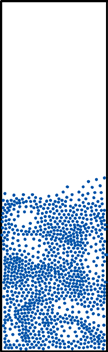
\includegraphics[width=0.8\textwidth]{35-11.png}\\
(a)
\end{minipage}
\begin{minipage}[t]{0.15\linewidth}
\centering
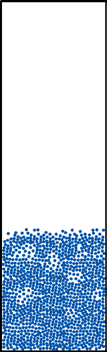
\includegraphics[width=0.8\textwidth]{35-12.png}\\
(b)
\end{minipage}
\begin{minipage}[t]{0.15\linewidth}
\centering

\includegraphics[width=0.8\textwidth]{35-13.png}\\
(c)
\end{minipage}
\begin{minipage}[t]{0.5\linewidth}
\centering
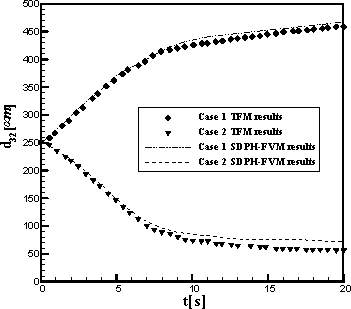
\includegraphics[width=0.9\textwidth]{35-14.pdf}\\
(d)
\end{minipage}
\caption{The spatial distribution of particles under different conditions. (a) No polymerization and breakup; (b) Case 1; (c) Case 2; (d) Curves of sauter diameter $d_{32}$ over time in case 1 and 2.}\label{fig:35}
\end{figure}

\end{abstract}


%%THE END OF ABSTRACT

\addbib

\end{document}
